%*****************************************
\chapter{Theory and Alternatives}\label{ch:theory_and_alternatives}
%*****************************************


\section{Feedback Control Model for Accomplishing a Single Goal}

\begin{figure}[bth]
  \center
  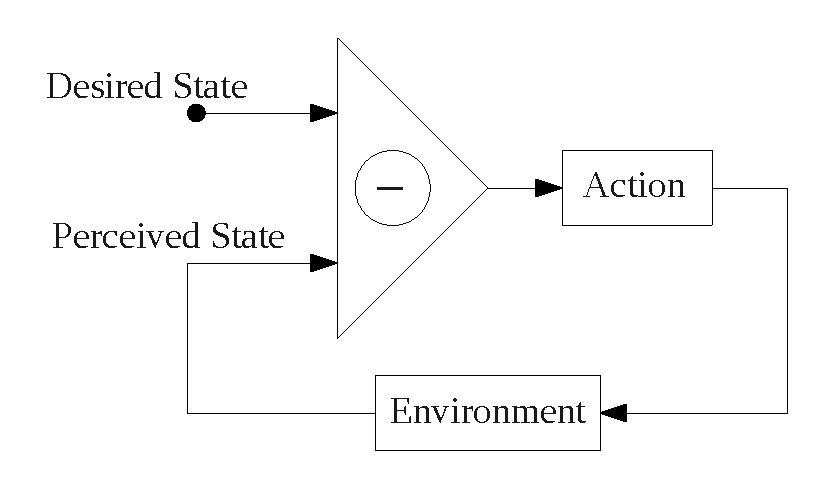
\includegraphics[width=6cm]{gfx/feedback_control}
  \caption[The feedback control model for accomplishing a single goal]{The feedback control model for accomplishing a single goal.}
  \label{fig:feedback_control}
\end{figure}

Now that we have discussed the basic model of learning from experience
what good goal states may be from rewards, let us consider the
representations for the state space of the perceptions and actions of
our model.  Control theory has given us many useful models for agents
that control continuous environments.  For example,
Figure~\ref{fig:feedback_control} shows a simple difference feedback
control circuit that is used in simple linear control systems.  The
system is given a desired state, there is a difference device that
calculates the difference between the actual perceived value from the
environment, and the control system then executes an action based on
that difference, which affects the environment.  The result in such a
negative feedback loop is that the agent's perception of the
environment is closer to the desired state.

\section{Means-End Analysis}

In 1959, Newell, Shaw, and Simon published a report on a means-end
analysis model that was designed to solve any symbolically represented
problem \citep{newell:1959}.  Their system was called the \ac{GPS},
and worked by being able to work with relational representations of
current and desired states.  The agent had a catalogue of differences
between states that it knew how to minimize.  The system worked by
finding the largest difference and executing the associated method for
reducing this difference.  This work has grown into the Soar model
\citep{newell:1990} for better solving symbolic planning problems, and
dealing with impasses for when the planning search runs out of
options.

\section{Difference-Engine Model for Accomplishing Multiple Goals}

\begin{figure}[bth]
  \center
  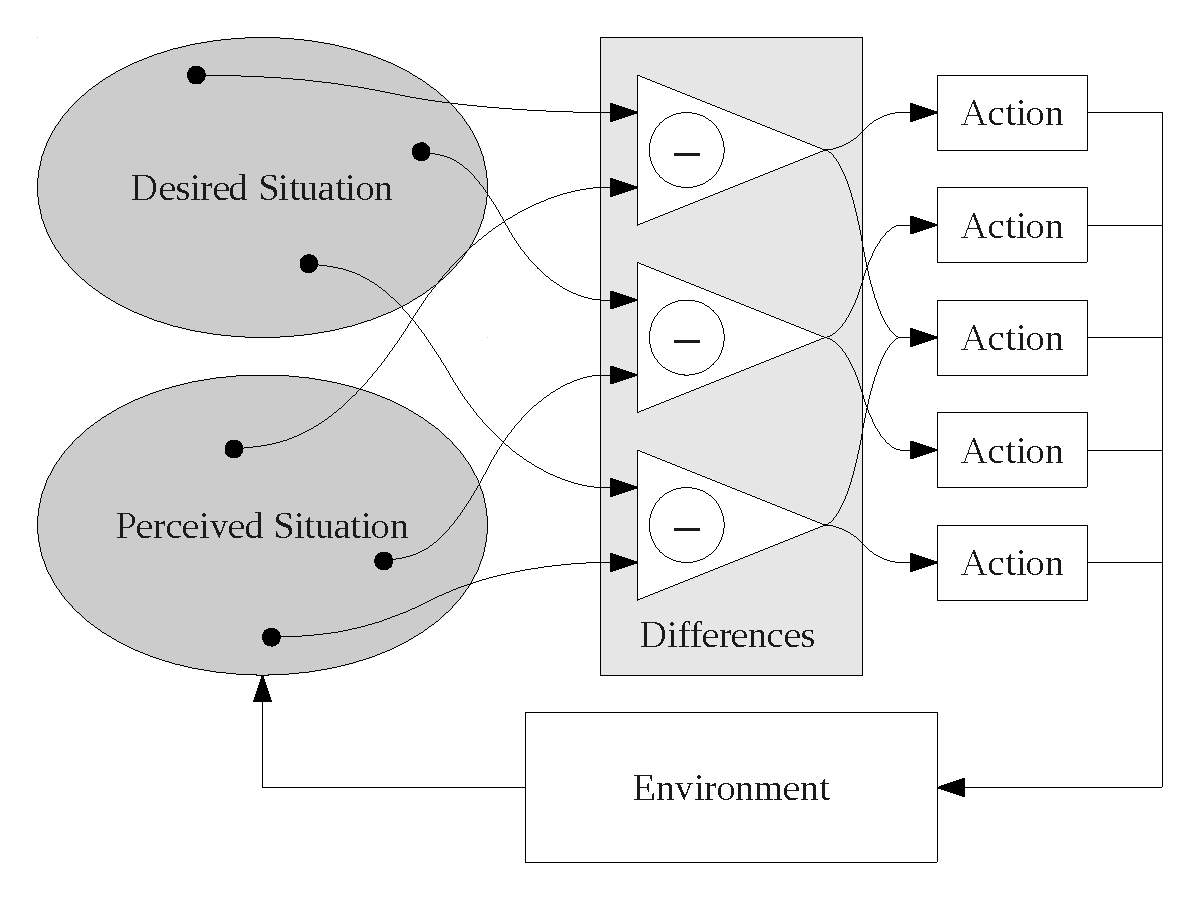
\includegraphics[height=6cm]{gfx/difference_engine_feedback_control}
  \caption[The difference engine model for accomplishing multiple goals]{The difference engine model for accomplishing multiple goals.}
  \label{fig:difference_engine_feedback_control}
\end{figure}

\citep[p.~78]{minsky:1988}


\section{EM-ONE}

We worked with Pushpinder Singh from 1999 to 2006 on the first version
of the Emotion Machine architecture, EM-ONE \citep{singh:2005}.
During that period, we discussed that one weakness in the EM-ONE
system is its reliance on tracing only the declarative prolog
statements, among other necessary but untraced procedural code.
Although EM-ONE contained a large amount of procedural knowledge, none
of the effects of this procedural knowledge could be debugged
reflectively.  Toward solving this problem, we have based our approach
on a memory layer that can trace the provenance of select memory
events.

